% !Mode:: "TeX:UTF-8"

\BiChapter{超密集组网的网络架构和系统模型}{architecture and system model}


超密集组网技术是5G中的关键的技术,用于满足大量用户的区域内,用户的高速率传输的需求。
密集热点区域无线网络场景下,由于系统中的用户较多,容量需求大,因此,需要网络能够提供更高的单位面积的频谱利用率。
同时,通信已经成为世界上最耗能的应用,因此要想办法在满足用户要求的同时,尽可能的降低能耗,从而得到较高的能耗比,即网络需要有很高的单位面积能量谱效率。

本章首先介绍了超密集组网的定义,接着结合超密集组网的网络的基本特性,介绍超密集组网场景中可能用到的网络架构,其中包括异构网络、CRAN架构和基于软件定义无线网络的架构,最后超密集组网的重要的性能指标。
为接下来的理论分析和算法优化打下基础。

\BiSection{超密集组网的定义}{Defination of UDNs}
超密集组网(UDN)作为~5G~的关键技术之一,对其概念的描述,网络布置的探索,再到性能分析、具体干扰管理算法的研究,随着对~5G~标准的不断探索,这些方面的研究也越来越深入。
未来通信系统服务需求的增加,且需要满足更好的用户体验,系统容量的增加就显得日益迫切。

根据现有的研究结果进行分析,超密集组网~UDN~在~5G~中的定义是:发射功率较低的小型的接入点,网络的拓扑结构不做精确的规划要求,网络中基站的密集程度很高的区域部署,即可以构成一个超密集网络\citeup{5Gwhitebook}。
采用超密集组网技术,发射机和接收机之间的距离大大降低,减少了路径损耗,单位面积内可以服务的用户量大大增多,提高频谱效率,小区中的流量的分配更加灵活,有效的提升了网络效率\citeup{spsharing} 。
总结来说,超密集组网就是通过提高单位面积频谱效率的方式来提高整体的系统容量。
超密集网络中单个小区提升系统容量的方式又分为以下两种:其一为增加带宽,为现有网络提供新的频谱资源;
其二为使用 Massive MIMO、高阶调制等方式提高每个小区的频谱效率。
超密集组网的网络部署方式仍处于探索阶段,但有几点已经达成共识。
第一,单一层次的蜂窝网部署方式无法满足 5G 移动通信系统的通信需求,多层次、多种接入方式并存的无线接入网络(Heterogeneous and Small Cell Networks, HetSNets)
是蜂窝网发展的必然趋势。
多层次是指传统宏小区(Macrocell)和包括微小区(Picocell)、家庭小区(Femtocell)、中继(Relay Nodes)在内的低功耗小区共存的体系结构。
除了传统蜂窝网接入方式以外,也包括无线局域网、无线个域网等多种接入技术。
第二,办公区域、居住区域、旅店商场等室内热点区域以及机场等室外热点区域需要高密度的小区部署,从而支持满足 QoS 要求的用户服务。
第三,除了手机等蜂窝网用户设备(UE)以外,还需要支持机器间通信,这种通信
业务也要与核心网络相连。
同时,对于大量的微小基站的接入,光纤和无线都应该被认为是合适的传输资源。

UDN 需要以非常灵活的方式来使用各类传输资源,如有线传输,无线传输,或混合传输,这样才能从时域,频域,空域等各个维度来全面地利用传输,以达到对资源的最大使用效率。
UDN 的网络拓扑结构应该是灵活的,以便动态地适应各种热点地区的部署,适应大量网络节点的接入,并适应多种无线技术。
因此,先进的自配置算法将被大量地使用在 UDN 网络中,以获得自动的小区参数配置,自动容量优化,自动负载平衡,自动资源分区及自主协调等能力。

\BiSection{超密集组网的网络架构}{The construction of UDN}
本小节中介绍超密集组网网络架构中较有潜力的,可以被应用的具有前景的网络架构,其中包括异构网络架构、CRAN架构和SDN架构。

\BiSubsection{异构网络}
超密集无线异构网络融合多种无线接入技术(如5G、4G、UMTS、Wi-Fi等),由覆盖不同范围、承担不同功能的大/小基站在空间中以极度密集部署的方式组合而成的一种全新的网络形态。
在超密集无线异构网络中,多种无线接入技术共存,大/小基站多层覆盖,既有负责基础覆盖的在传统蜂窝网络中所使用的宏基站, 也有承担热点覆盖的低功率小基站,如micro、pico、relay、femto等。
为了解决1 000倍容量挑战,为用户提供极致化的业务体验,未来实际部署的超密集无线异构网络会远远超出现网的布设密度和规模。
据预测, 在未来无线网络中,在宏基站的覆盖区域中,各种无线传输技术的各类低功率节点的部署密度将达到现有站点部署密度的10倍以上,站点之间的距离将降至10m甚至更小,支持高达25 000个用户/km$^2$,甚至将来激活用户数和站点数的比例达到1:1,即每个激活的用户都将有一个服务节点。

广义的异构网络是指存在多种无线接入技术(Radio Access Technology,RAT)的混合型网络,包括 LTE 网络、5G 网络、WIFI 网络、个域通信以及物联网等。
LTE 提出了狭义的异构网络概念,即 LTE 系统内的 HetNet,实现在一个目标区域内重叠部署不同类型的小区,如在一个宏蜂窝小区覆盖范围内部署多个家庭小区和微微蜂窝小区等。
Micro eNB、PeNB、HeNB、Relay 等的部署可以降低站点获取难度,解决覆盖忙区、盲区的问题。

微蜂窝 Micro 小区发射功率和覆盖半径比 Macro 小区小,用于密集城区局部区域的深度覆盖,作为街道站应用。

微微蜂窝 Pico 小区可以用来增加对非对称用户分布小区热点区域的覆盖。
微微基站可以看成一个发射功率较低、覆盖范围较低的宏基站,微微基站可以和宏基站在覆盖区域上相互重叠。部署微微基站需要重新设计射频信号强度和质量相关的算法、过程和参数,以及优化切换流程,实现网络负载均衡。

毫微微蜂窝,即家庭基站小区,主要服务于家庭用户,它可以通过用户的宽带拨号或者 HeNB 网关接入核心网,家庭基站可以部署在较高的频段,提高高频段频谱资源的利用率。
家庭基站是属于用户私有的付费基站,各种参数配置和宏基站之间很难进行协调操作,干扰管理、资源分配、基站切换、接入控制等难题亟待解决。

中继节点 Relay 和普通基站一样为用户提供无线接入,有独立的小区标识,是基站和用户之间中专数据和信令的节点,用于保证广覆盖,同时也能减少部署基站的成本。
Relay 有两种模式,若基站到 Relay 的链路使用的频率和 Relay 到用户使用的相同,则称为带内中继(Inband Relay;
若基站到 Relay 的链路使用的频率和 Relay 到用户的链路不同,则称为带外中继(Outband Relay)。Relay 技术实现较为复杂,但是节省传输,安装灵活方便。

分布式天线系统,即无线射频拉远(Remote Radio Head,RRH),包括基带控制单元和射频拉远单元,可以根据不同环境构建链型、树型、环型、星型结构的网络,增强网络部署的灵活性。

异构网络的架构如图所示。

\BiSubsection{CRAN}{CRAN}
C-RAN架构最大的特点是基带资源池化特性,基带资源可以在不同的基站之间共享。
基于虚拟基带处理单元池和遥控射频端的联合,相比于其他的蜂窝网络,C-RAN架构有更低的网络延时。
根据LTE的协议栈,C-RAN架构一共有L1,L2,L3三个层级,L1为物理层,主要功能是实现信道编码、速率匹配、MIMO以及为高层提供数据传输服务。
L2层负责媒体接入控制、射频链路控制以及主要提供数据链路控制的分组数据汇聚协议(PDCP)。L3层是射频资源控制(RRC)层,主要提供信令和射频资源控制。
根据L1层的位置可以把C-RAN架构分为两种。分别是“全中心化(full centralization)”和“部分中心化(partial centralization)”。
其中“全中心化”架构将L1、L2、L3三层全部放在了基带信号处理单元池端。“部分中心化”将L1层与遥控射频头相结合。
二者的共同点是均需要强大的前向回传链路为其提供高速的发送速率。虚拟的基带信号处理单元池和云端的基站负责限制射频信号的发送和接收。
遥控射频头用来收集和管理来自终端信号通过数字信号处理(DSP)控制器。
在第一种架构中,所有的C-RAN层结构和基带功能全部整合到基带数据处理单元池当中。
由于协议存储在虚拟的基带数据处理单元池中,该架构的协议层对安全威胁有更好的抵抗能力,如窃听和干扰攻击、身份盗窃攻击等,同时也使用户接入控制、频谱分配和连接建立更加的便捷。
除此之外,基于虚拟的基带数据处理池,多标准的数字信号可以灵活有效地被多小区协作信号处理技术分类。
在第二种架构中,仅整合协作功能、L2、L3层的调度和无线资源分配到基带数据处理单元池当中。
该架构调度可以感知到物理层的联合传输和联合发送,从而合适地调度频谱资源来提升小区边缘的性能。该架构与当前的4G网络架构类似,可以使现存的传输网络改变最小。
C-RAN现在也代指具有云化、中心处理、共享频谱、协作、清洁性质的网络架构。

CRAN是干扰协调和频谱资源管理的有效的方法。由于RRH结构简单,RRH可以以较低的硬件成本进行密集的布放,BBU池化后资源统一调度,能量效率更高。
由于中心化的架构,多用户干扰可以被诸如CoMP这样的多点协作技术有效的解决掉,这样将会有很有效的性能增益。
在传统的CRAN架构中(4G),C-RAN被部署用于连接宏基站和BBU池,由于BBU和RRH之间的传输路径长,这种传统的基站会造成很大的传输时延,而在密集热点区域采用C-RAN架构,延迟也会被大大的缩短。
不仅如此,它还是有效解决潮汐效应的一种方式。

但CRAN架构也不是完美的。若要将CRAN架构应用与超密集组网当中,需要减小功耗,建立RRH睡眠与活跃状态的选择机制。
不仅如此,还要实现低花费的前向链路,因为前向链路能够提供的能量资源是有限的。
同时也要降低网络中算法的复杂度,降低训练开销。

CRAN~网络架构如图~\ref{CRAN}~所示。
\begin{figure}[htbp]
\centering
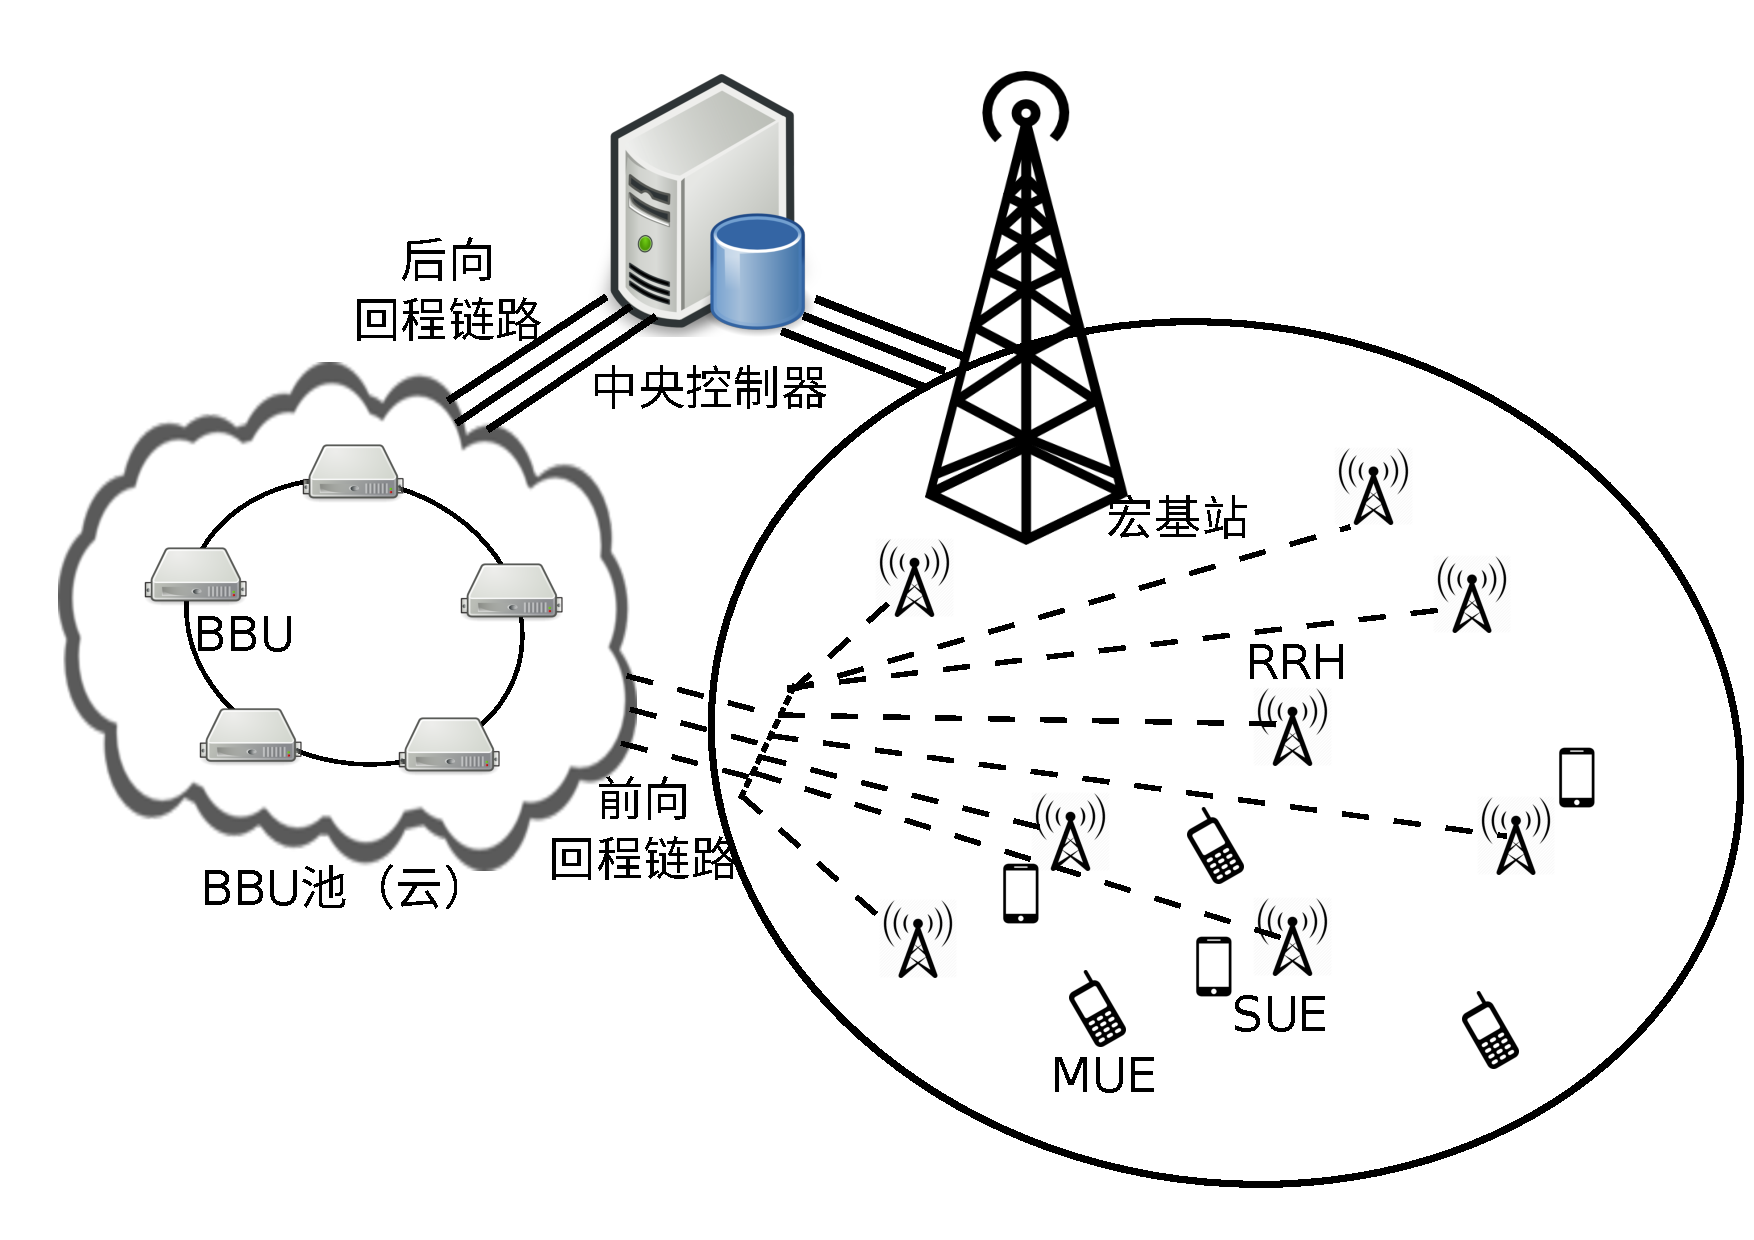
\includegraphics[width = 0.62\textwidth]{H-C-RAN_PPP.pdf}
\caption{CRAN~网络架构的示意图}\vspace{-1.5em}
\label{CRAN}
\end{figure}

可以看到图中,CRAN架构分为三个主要部分:BBU池、中央控制器和RRH。其中BBU池和中央控制器通过后向回程链路相连接,BBU池和RRH通过前向回程链路相互连接。
其中小区中包括宏基站,为了满足网络中的大连接和高速率,小区中还布置了很多微基站,微基站的数据通过前向回程链路传至BBU池做基带信号的处理。
通过中央控制器完成网络层的协议,如小区切换,跨区访问等等。

\BiSubsection{软件定义无线网络}{SDWN}

为了应对封闭、僵化、难以在传输速率和容量上做出突破的传统网络,研究者提出软件定义网络(Software-DefinedNetworking,SDN)的概念,SDN将控制功能从数据转发层中分离出来,使得终端接入、数据转发等功能统一由控制器控制,同时开放网络设备的可编程接口,提高了网络的灵活性和可控性。
SDN与无线网络相结合,形成软件定义无线网络(Software-DefinedWirelessNetworking,SDWN)。
SDWN相对于原有的无线网络架构,是对原有无线网络技术的全面升级,而不是简单的将控制平面与数据平面分离。主要体现在如下几个方面:

(2)~切换管理

切换管理一直是无线通信中的重点和难点。由于终端节点的移动将引起节点切换问题。
同时,在SDWN网络中,随着网络控制功能的丰富,终端会因为各种不同的部署进行切换,在使用不同业务时可能也涉及到节点切换问题。
节点切换的速度以及切换前后用户得到服务的变化,是SDWN性能评价的重要指标之一。

(2)~负载均衡

SDWN中,AP的负载能力有限,若单个AP上有过多的业务时,则会使AP过载,从而无法保证服务质量。
针对此问题,软件定义无线网络提出,当某一区域内同时包含有负载较小和较大的AP时,控制器应将更多客户端(包括已经连接到负载较大AP上的)接入到负载较小的AP。
也可以让控制器在获取网络状况(拓扑结构、负载等)的同时,可以重定向服务请求,为终端选择更加适合的服务器,实现流量均衡。

(3)~无线网络虚拟化

为了解决当前互联网面临的固有的问题传统的网络虚拟化技术以虚拟局域网(Virtual Local Area Network, VLAN)与虚拟专用网(Virtual Private Network,VPN)为代表,通过协议封装在物理网络上提供互相隔离的虚拟专用网络。
近年来,网络虚拟化已扩展到移动和无线网络的情况下,形成了无线网络虚拟化(Wireless Network Virtualization,WNV)。
WNV中,物理节点和物理链路被虚拟化为不同虚拟网络的虚拟节点和虚拟链接。
SDWN解耦控制层面与数据平面,引入控制中心化,这些思想可以显著提高WNV的可编程性和定制性,同时为WNV提供最优的控制和操作策略。
另一方面,虚拟化思想增强了网络的灵活性和伸缩性,能大幅提高SDWN的网络资源利用率。因此,虽然WNV和SDWN的研究动机、目标、技术细节、实现方法等不尽相同,但WNV与SDWN高度互补,为未来的移动和无线网络研究指明了方向。

\BiSection{超密集组网通信的性能指标}{matrices}
超密集组网的网络部署方式仍然处于探索阶段,但采用异构网络的方式已经达成共识。单一层次的蜂窝网部署方式无法满足 5G 的通信需求,多层次、多种接入方式并存的无线接入网络(Heterogeneous and Small Cell Networks,HetSNets)是蜂窝网发展的必然趋势。
多层次是指传统宏小区(Macrocell)和包括微小区(Picocell)、家庭小区(Femtocell)、中继(Relay Nodes)在内的低功耗小区共存的体系结构。

\BiSubsection{信干噪比}{SINR}

可靠性和有效性一直是评定通信性能的一个重要指标。其中有效性可以通过网络的信道容量进行衡量。而网络的信道容量是一个直接与信干噪比有关的量。
信干噪比的表达式如~(\ref{SINR})~所示:
\begin{equation}\label{SINR}
  \mathrm{SINR}=\frac{S}{I+N}
\end{equation}
其中~$S$~为通信链路中接收机的接收功率,~$I$~为其他的通信链路对该通信链路所造成的干扰。$\mathrm{SINR}$~表示该通信链路的信干燥比。

超密集组网区域用户与基站之间距离比较近,因此干扰占有几乎全部的比重,反之噪声的影响几乎可以忽略不计。也就是说,密集无线网络是一个干扰受限的信道。其信干比近似等于信干燥比。信干比的表达式如~(\ref{SIR})~:
\begin{equation}\label{SIR}
  \mathrm{SIR}=S/I
\end{equation}
其中~$\mathrm{SIR}$~表示该通信链路的信干比。
\BiSubsection{用户的遍历容量}{ASE}
给定一个用户的接收信干比,即可以求出一个用户的遍历容量,在平稳的瑞利信道下,用户的遍历容量如式~$\ref{e_capacity_formular}$~所示:
\begin{equation}\label{e_capacity_formular}
  C_{Rayleigh} = \int_{0}^{\infty} B \log_2(1+\mathrm{SINR}(h)) f(h) \mathrm{d} h
\end{equation}
其中~$C_{Rayleigh}$~为瑞利信道的遍历容量,~$f(h)$~为~$h$~的概率密度分布函数,$B$~为信道的带宽。信道的遍历容量表示一个用户在一段时间内,遍历所有可能性下的信道容量的统计平均值。
因为信道为瑞利信道,因此在固定位置上的用户,由于受到了信道系数的影响,其信干噪比在不同的时间点上也是不同的,又由于瑞利信道是平稳的信道,
因此可以采用遍历所有信道系数的可能性得到的统计均值代替时间上的遍历,用~$\mathrm{SINR}(h))$~表示。

遍历容量可以反应一个用户在一段时间内通信的有效性,是反应网络性能的重要指标。

\BiSubsection{区域覆盖率}{Coverage}
为保证用户的服务质量与速率要求,用户的接收信干比需要维持在一个固定的门限上,而到底有多少用户在该时刻上有很好的信干比,或者说在瞬时上能达到所要求的信干比的用户一共有多少呢?区域覆盖率是评定的有效的指标。
区域覆盖率的定义如~(\ref{pc})~所示:
\begin{equation}\label{pc}
  p_c(T) = \mathbb{P}[\mathrm{SINR}>T]
\end{equation}
其中~$T$~为给定的信干噪比的门限,~$\mathrm{SINR}$~为通信链路的信干噪比,$\mathbb{P}$~表示概率。根据定义,可对其物理意义做出以下的三种解释:

 (1)~服务用户的信干噪比为以上的概率。

 (2)~信干噪比为以上的用户占总用户的百分比。

 (3)~信干噪比为以上的区域占总区域的百分比。

覆盖率是评定无线网络性能的一个重要的概念,并且根据覆盖率,可以很容易的得到有能达到给定的速率要求在整个区域中的所有用户的占比。
同时该物理量也是单位区域上信干噪比的概率分布函数的补函数。
\BiSubsection{区域面积谱效率}{ASE}

香农定理给出了通信系统的理论容量上界\citeup{TheMathematicalTheoryOfCommunication},表达式如~(\ref{shannon})~所示:
\begin{equation}\label{shannon}
  C = B \log_2(1+\mathrm{SINR})
\end{equation}

式~(\ref{shannon})~中,~$C$~ 代表理论的容量的上界也即系统最大的传输速率, $B$ 代表信道的带宽, ~$\mathrm{SINR}$~ 代表接收端信号的信干噪比。
香农定理可以解释现代各种无线制式由于带宽不同,所支持的单载波最大吞吐量的不同。香农公式表达了在给定带宽下,噪声和干扰都服从高斯分布的情况下,系统所能达到的理论最大容量。

频谱效率的定义为单位带宽上所能承载的最大的吞吐量,如~(\ref{SE})~所示:
\begin{equation}\label{SE}
\eta_{SE}=C/B=\log_2(1+\mathrm{SINR})
\end{equation}
上式中~$C/B$~就是单位带宽的容量,单位为~$bps/\mathrm{Hz}$~体现信道链路的传输性能。式~(\ref{SE})~给出了理论上频谱效率的理论最大值。

在密集热点区域无线网络的场景中,单个链路的容量已经不再是衡量一个网络的好坏的唯一指标,在超密集热点区域无线网络的场景中,还要考虑在一段时间内,网络中服务的用户的和容量。
同时,考虑到不同区域上的频谱效率相差可能非常悬殊。因此在密集热点的网络环境下,频谱效率将不能够完全反映整个区域的无线网络的性能,
取而代之的是单位面积谱效率这一物理量,其定义为在单位面积上的频谱效率,表达式如~(\ref{ASE})~所示:
\begin{equation}\label{ASE}
  \eta_{ASE}=C/(B\cdot S) = \lambda\mathbb{E}[\log_2(1+\mathrm{SINR})]
\end{equation}
单位为~$bps/\mathrm{Hz}/\mathrm{m}^2$~。其中~$\lambda$~为服务区域内基站的密度。区域面积谱效率的物理意义为单位面积上所承载的平均的和容量。

\BiSection{本章小结}{Conclusion}
本章主要对超密集组网现阶段的研究基础进行了分析,为后续章节的深入分析打下基础。
首先给出了超密集组网的定义,在分层异构的网络架构下,通过部署高密度低功耗的节点,来极大的提升系统容量,达到下一代移动通信 5G 满足1000 倍速率提升的要求。
同时给出通信性能的衡量指标,一般通过区域频谱效率,区域能量效率,成本效率来衡量超密集组网。
核心性能指标和典型场景指标则从实用性的角度给出了系统需要符合的性能参数,对于实际系统的规划与部署具有指导意义。
为了进一步明确超密集组网的网络构架,多址接入技术以及实现大容量的可行性,本章的第三部分给出了超密集组网中的主要技术,大规模天线技术可以带赋形增益和频谱效率的提升;
新型的非正交稀疏码分多址技术 SCMA 可以在利用同等资源的情况下,接入更大量的用户,提升系统容量;
以去蜂窝网化为核心理念的 C-RAN 技术,可以进行信息的集中处理,降低能耗;
D2D 技术作为超密集组网中最具潜力的技术,使得大规模密集通信成为可能。
文章对这四种技术进行简要介绍和说明,确定在超密集组网中的使用方式,所能取得的性能优势。
